\chapter{Perceptual Experiments}
\label{chap:PerceptualExperiments}

\section{Reconstruction Individual Harmonics}
\label{sec:PerceptualExperiments-Reconstruction}
	An experiment was conducted to evaluate which harmonic excitation method is best suited to the generation of
	individual harmonics. A primary aim of this experiment was to determine whether any of the methods would cause a
	tone from a single instrument to be perceived as coming from multiple sources. Each method was used to reconstruct
	signals which from which some harmonic content had been removed. The quality of the reconstruction was assessed by
	participants in a multiple stimulus listening test. 

	The audio samples each consisted of a single instrument playing a sustained tone. The instruments used were:

	\begin{itemize}
		\item A bowed cello.
		\item A clarinet.
		\item A synthesised harmonic sound.
		\item A piano.
	\end{itemize}

	For each sample the third through ninth harmonics were removed. Spectrograms of the cello sample before and after
	this process are shown in Figures \ref{fig:CelloSpectrogram} and \ref{fig:CelloFilteredSpectrogram}.  Test stimuli
	were then created by reintroducing these harmonics using SSBA, IAP and a synthesis method.  The synthesis method
	consisted of using the STFT to measure the amplitude envelope of the fundamental frequency and applying this to a
	synthesised sine wave at the frequency of the desired harmonic. 

	\begin{figure}[h!]
		\centering
		\subfloat[Unprocessed Sample]
		{
			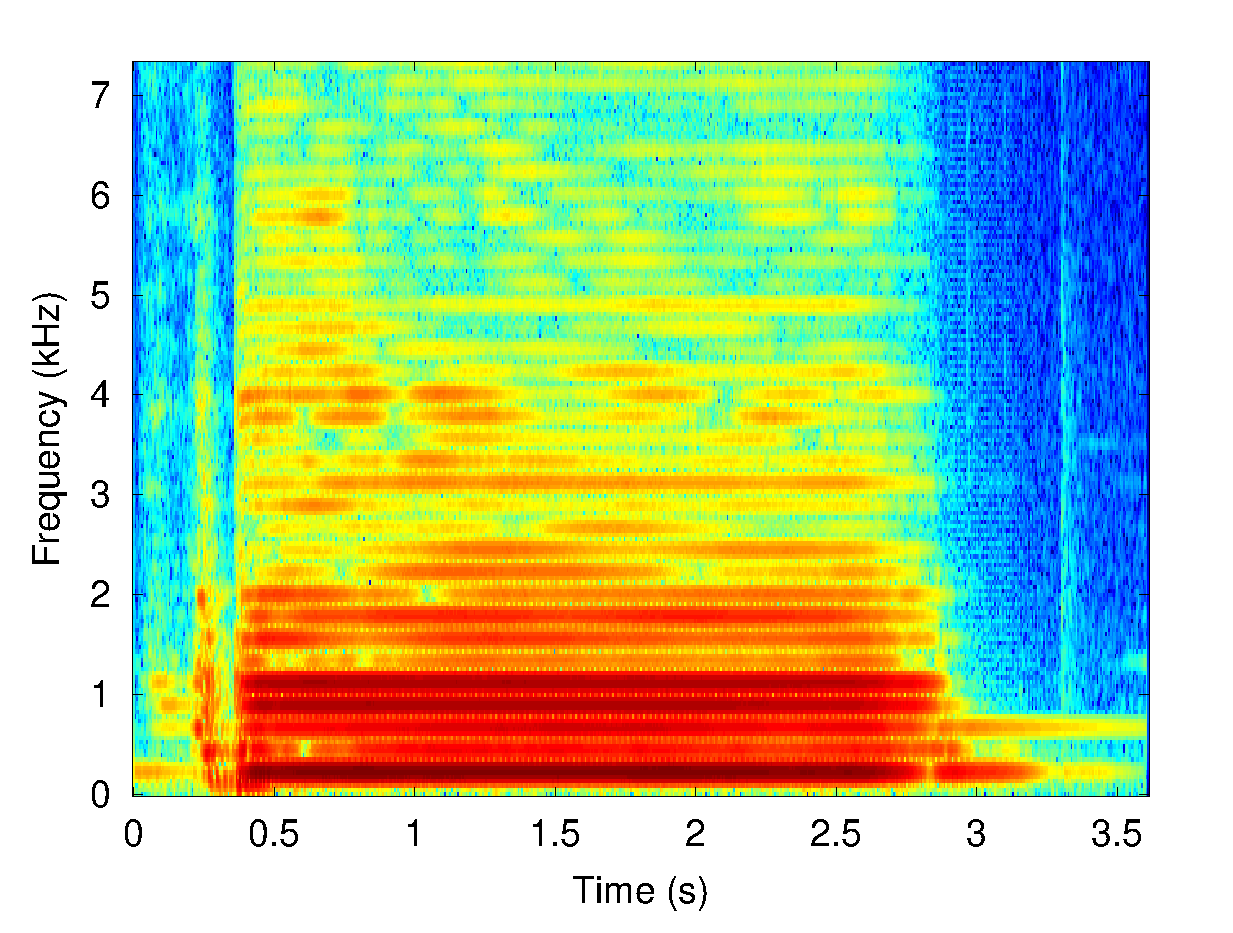
\includegraphics[width=0.45\textwidth]{chapter7/Images/CelloSpectrogram.eps}
			\label{fig:CelloSpectrogram}
		}
		\qquad
		\subfloat[Filtered Sample]
		{
			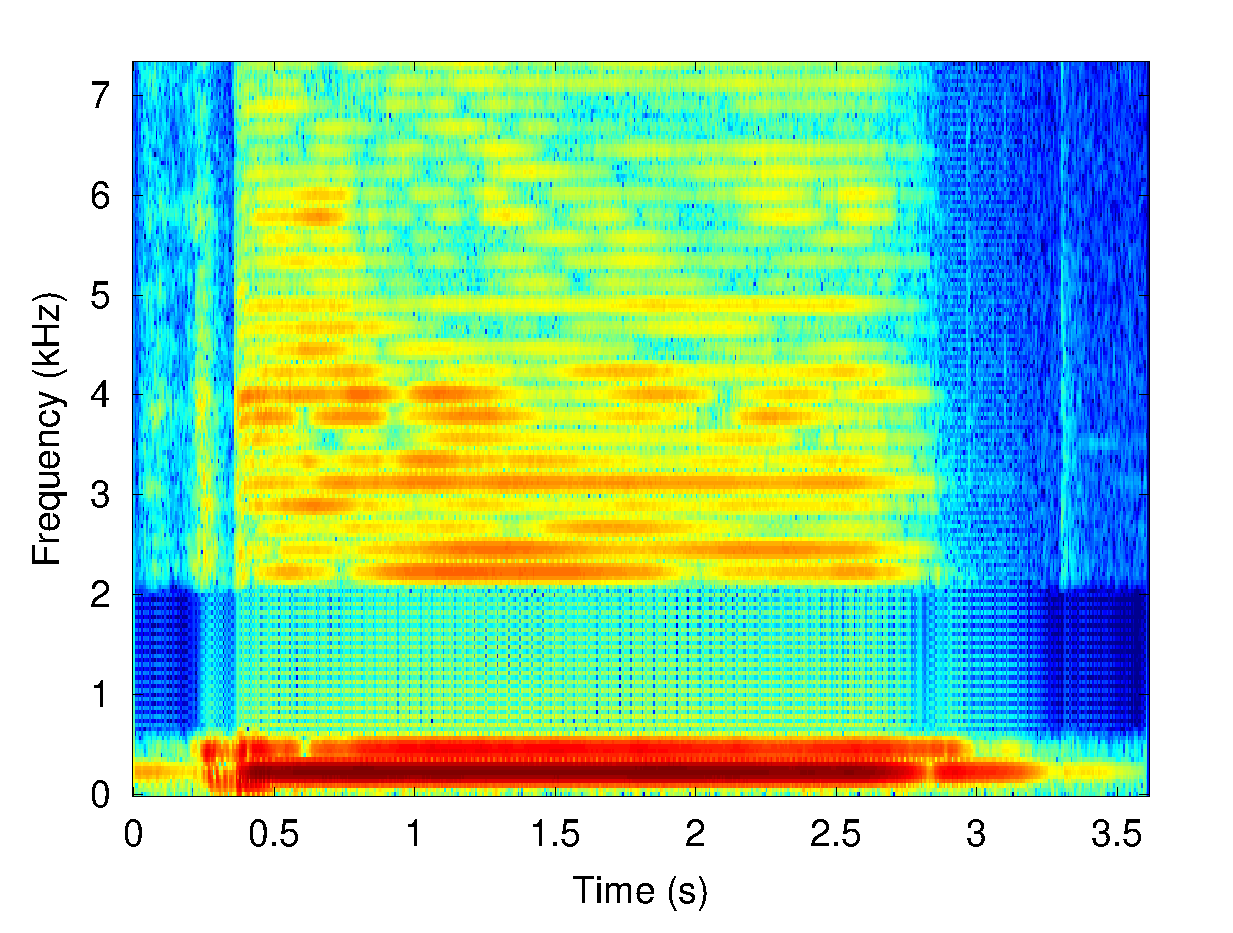
\includegraphics[width=0.45\textwidth]{chapter7/Images/CelloFilteredSpectrogram.eps}
			\label{fig:CelloFilteredSpectrogram}
		}
		\caption{Spectrograms of the cello sample.}
		\label{fig:CelloSpectrograms}
	\end{figure}

	Each sample was reconstructed three times using each method, using different parameters each time. For the SSBA and
	IAP methods a different order FIR filter was used to isolate the fundamental frequency. The filters used had orders
	of 50, 100 and 500. For the synthesis method the window length of the STFT was changed, taking values of 50, 100 and
	500 samples. Spectrograms for the reconstructed samples using the smallest filter order / STFT window length are
	shown in Figure \ref{fig:ReconstructedCelloSpectrograms}.

	\begin{figure}[h!]
		\centering
		\subfloat[SSBA with a 50\super{th} order filter.]
		{
			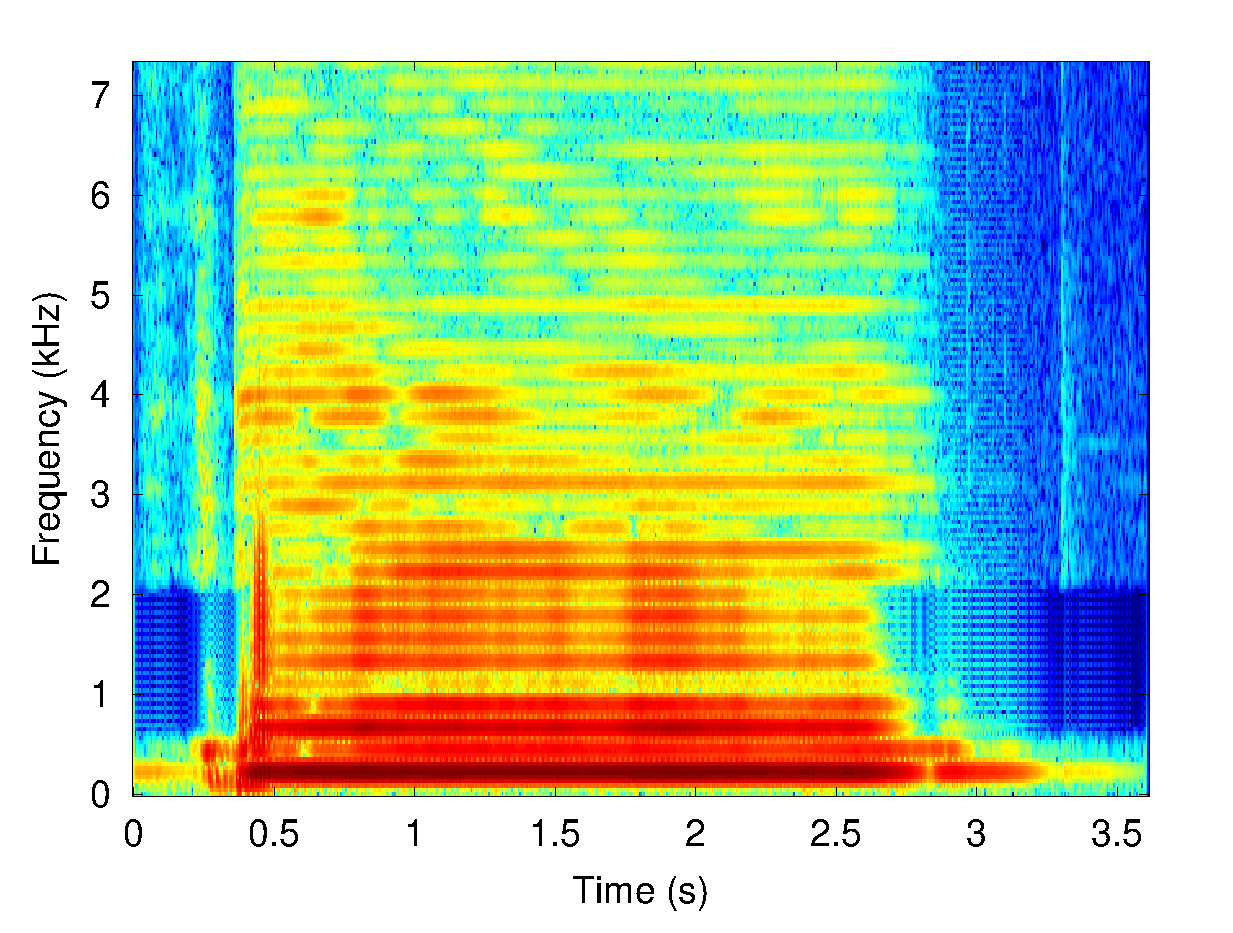
\includegraphics[width=0.45\textwidth]{chapter7/Images/CelloSSBASpectrogram.eps}
			\label{fig:CelloSSBASpectrogram}
		}
		\qquad
		\subfloat[IAP with a 50\super{th} order filter.]
		{
			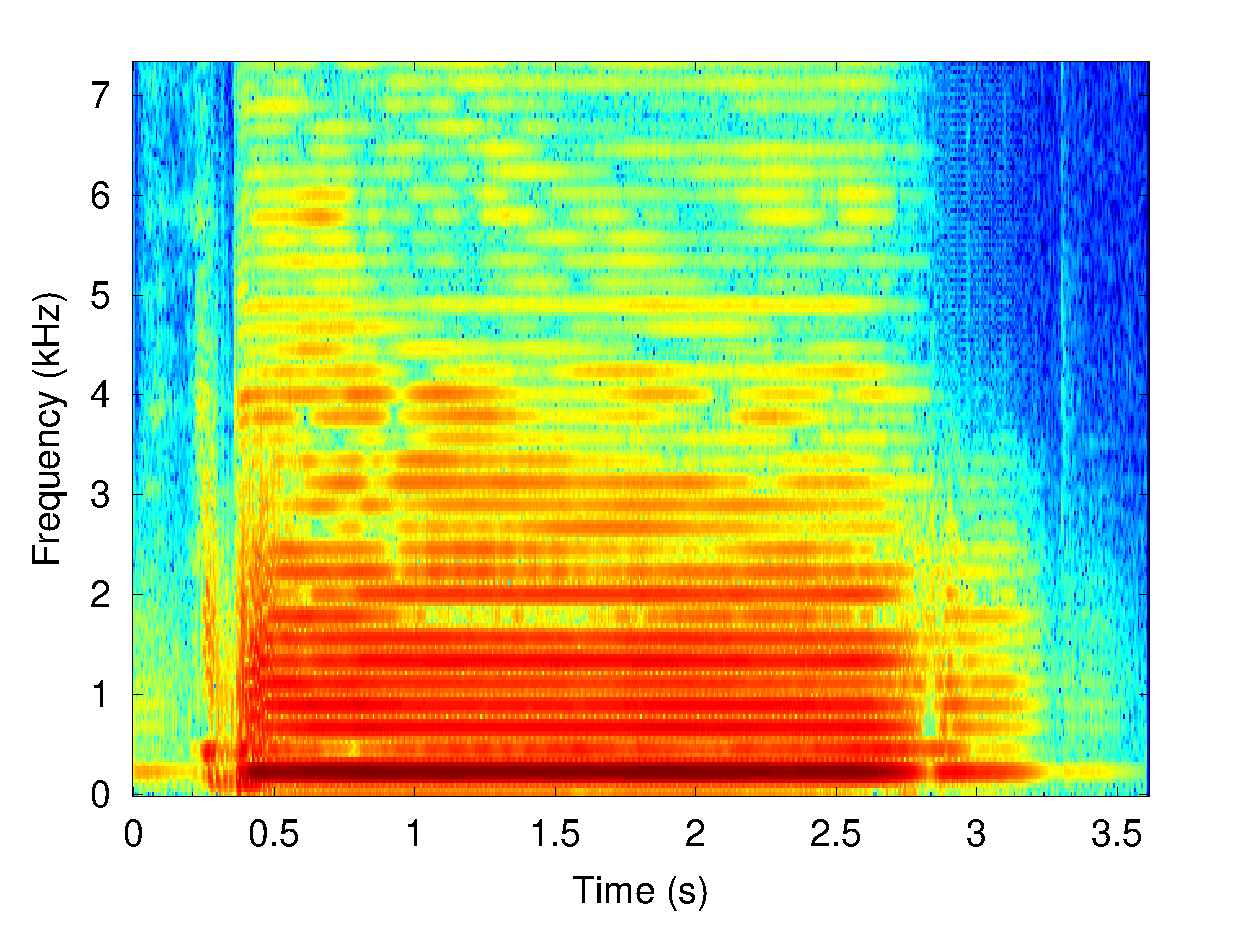
\includegraphics[width=0.45\textwidth]{chapter7/Images/CelloIAPSpectrogram.eps}
			\label{fig:CelloIAPSpectrogram}
		}
		
		\subfloat[Synthesis with an STFT window length of 50 samples.]
		{
			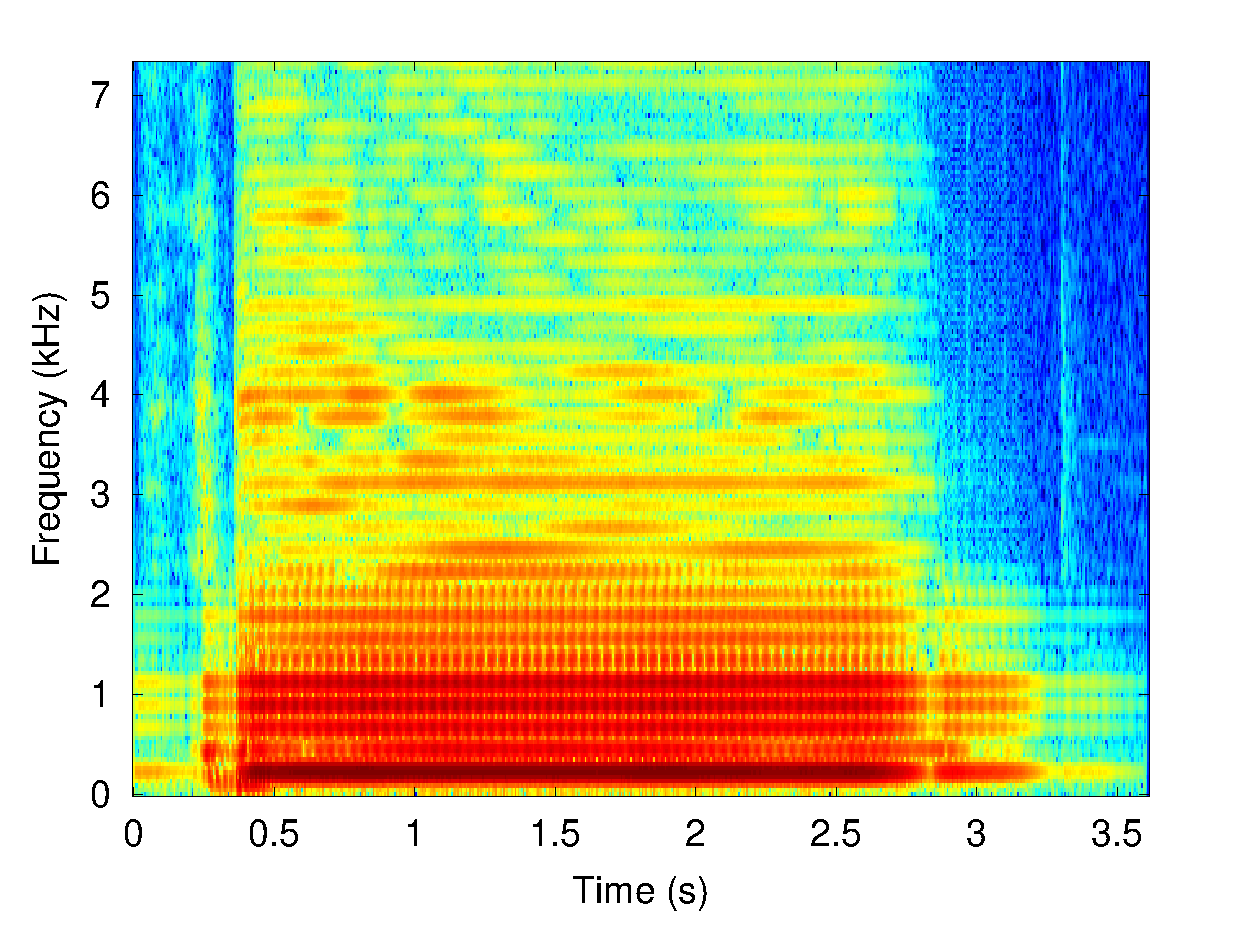
\includegraphics[width=0.45\textwidth]{chapter7/Images/CelloSynthesisSpectrogram.eps}
			\label{fig:CelloSynthesisSpectrogram}
		}
		\caption{Spectrograms of the cello sample reconstructed using three different methods.}
		\label{fig:ReconstructedCelloSpectrograms}
	\end{figure}

	On inspection of these spectrograms the characteristics of the three excitation methods can be seen. The amplitude
	envelopes of the generated harmonics differ greatly between the methods. Comparing the decay portion of the
	envelopes compared with those in the original signal (Figure \ref{fig:CelloSpectrogram}) highlights these
	differences. In the cello sample the fundamental frequency and third harmonic have a longer decay time then the
	other harmonics. The harmonics generated by the IAP and synthesis methods (Figures \ref{fig:CelloIAPSpectrogram} and
	\ref{fig:CelloSynthesisSpectrogram}) use the amplitude envelope of the fundamental frequency extending the decay
	time of the these harmonics compared to that in the original. Those generated by the SSBA method (Figure
	\ref{fig:CelloSSBASpectrogram}) have shortened decay times. As the order of the harmonic is increased the decay time
	gets shorter due to the dynamic expansion shown in Figure \ref{fig:SSBATemporalEffects}.

	The amplitude envelopes of the harmonics generated using the synthesis techniques exhibit a large amount of ripple.
	This is due to the amplitude of the fundamental being calculated in blocks. These inaccuracies are not present in
	the harmonics generated using the IAP method as the amplitude is calculated on a sample by sample basis.

	Test participants were presented with all processed version of a particular sample at once along with a reference
	stimulus (the unprocessed sample) and an anchor stimulus (the sample with its harmonics removed).  Participants were
	asked to grade how well each processed stimulus recreated the reference stimulus on a scale from 0 to 100.

	The results of this experiment are shown in Figure \ref{fig:SMCResults} with error bars showing the 95\% confidence
	intervals. The stimuli numbers refer to different processing algorithms as follows.

	\begin{tabular}{>{\bfseries}cl}
		1. & Reference Stimulus \tabularnewline
		2. & Sample reconstructed using the synthesis method with an STFT window length of 50
		     samples. \tabularnewline
		3. & Sample reconstructed using the synthesis method with an STFT window length of 100
		     samples. \tabularnewline
		4. & Sample reconstructed using the synthesis method with an STFT window length of 500
		     samples. \tabularnewline
		5. & Sample Reconstructed using the SSBA method using a 50\super{th} order filter. \tabularnewline
		6. & Sample Reconstructed using the SSBA method using a 100\super{th} order filter. \tabularnewline
		7. & Sample Reconstructed using the SSBA method using a 500\super{th} order filter. \tabularnewline
		8. & Sample Reconstructed using the IAP method using a 50\super{th} order filter. \tabularnewline
		9. & Sample Reconstructed using the IAP method using a 100\super{th} order filter. \tabularnewline
		10. & Sample Reconstructed using the IAP method using a 500\super{th} order filter. \tabularnewline
		11. & Sample with third through ninth harmonics removed (anchor). \tabularnewline
	\end{tabular}

	\begin{figure}[h!]
		\centering
		\subfloat[Cello Sample]
		{
			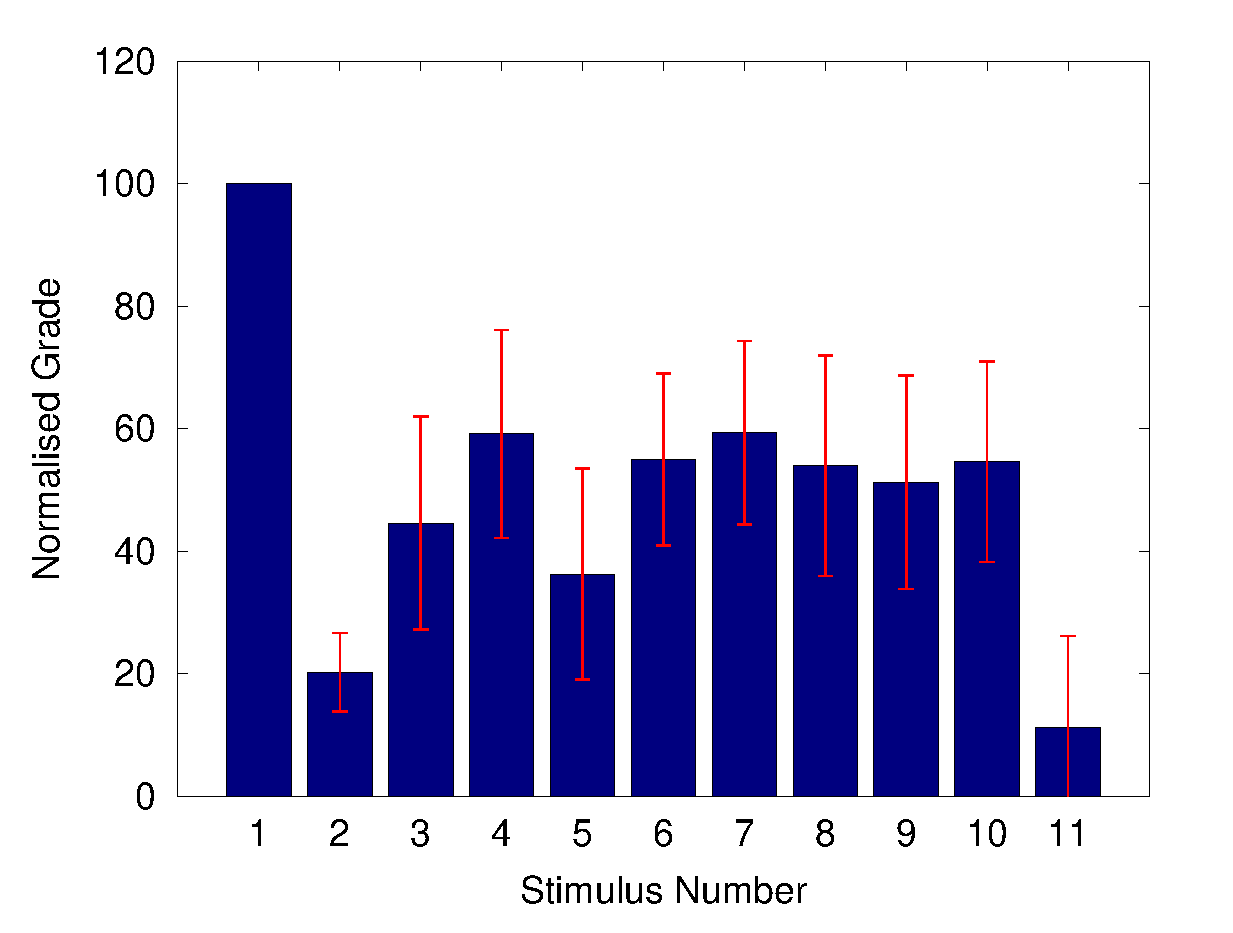
\includegraphics[width=0.45\textwidth]{chapter7/Images/CelloResults.eps}
			\label{fig:CelloResults}
		}
		\qquad
		\subfloat[Clarinet Sample]
		{
			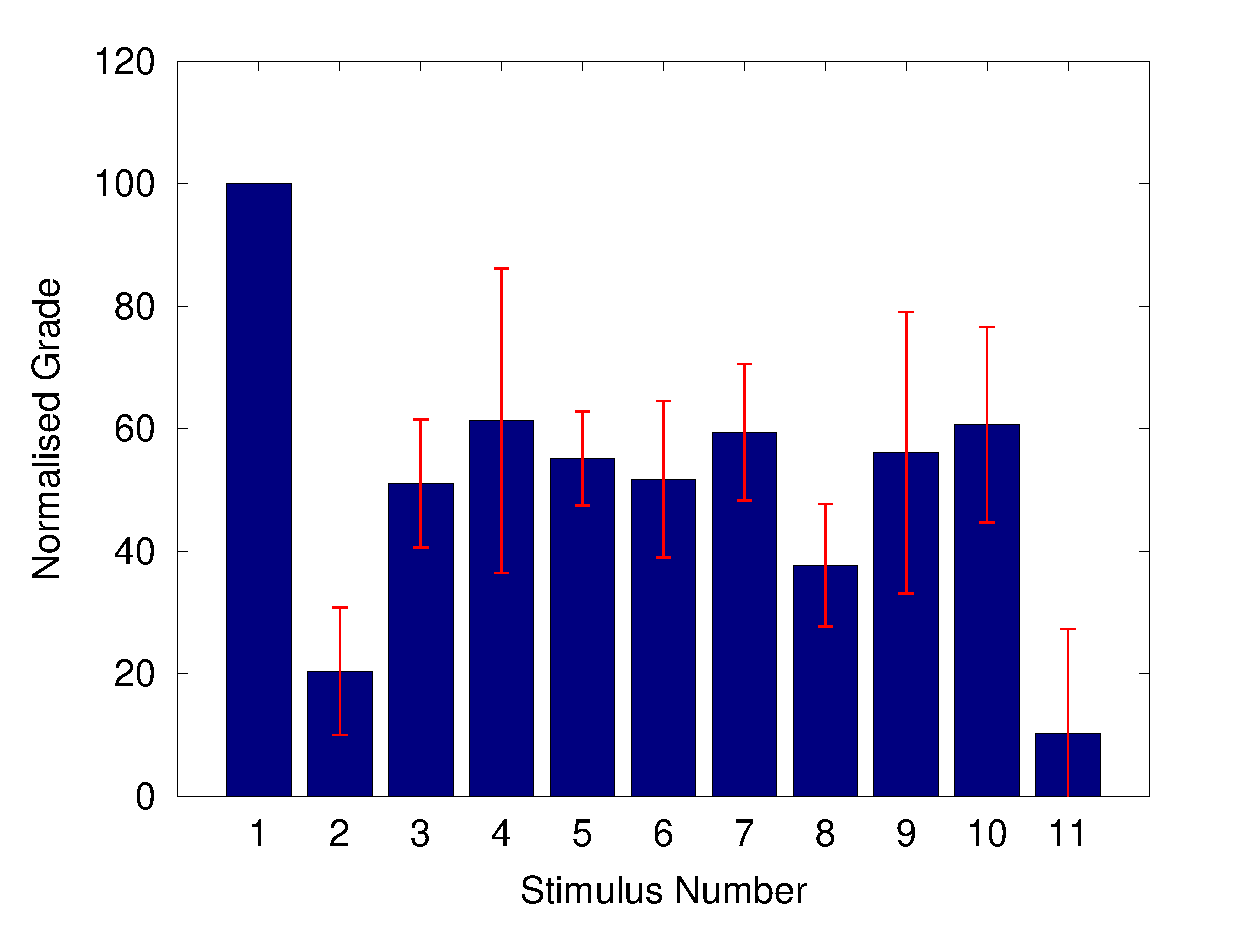
\includegraphics[width=0.45\textwidth]{chapter7/Images/ClarinetResults.eps}
			\label{fig:ClarinetResults}
		}

		\subfloat[Synthesised Sample]
		{
			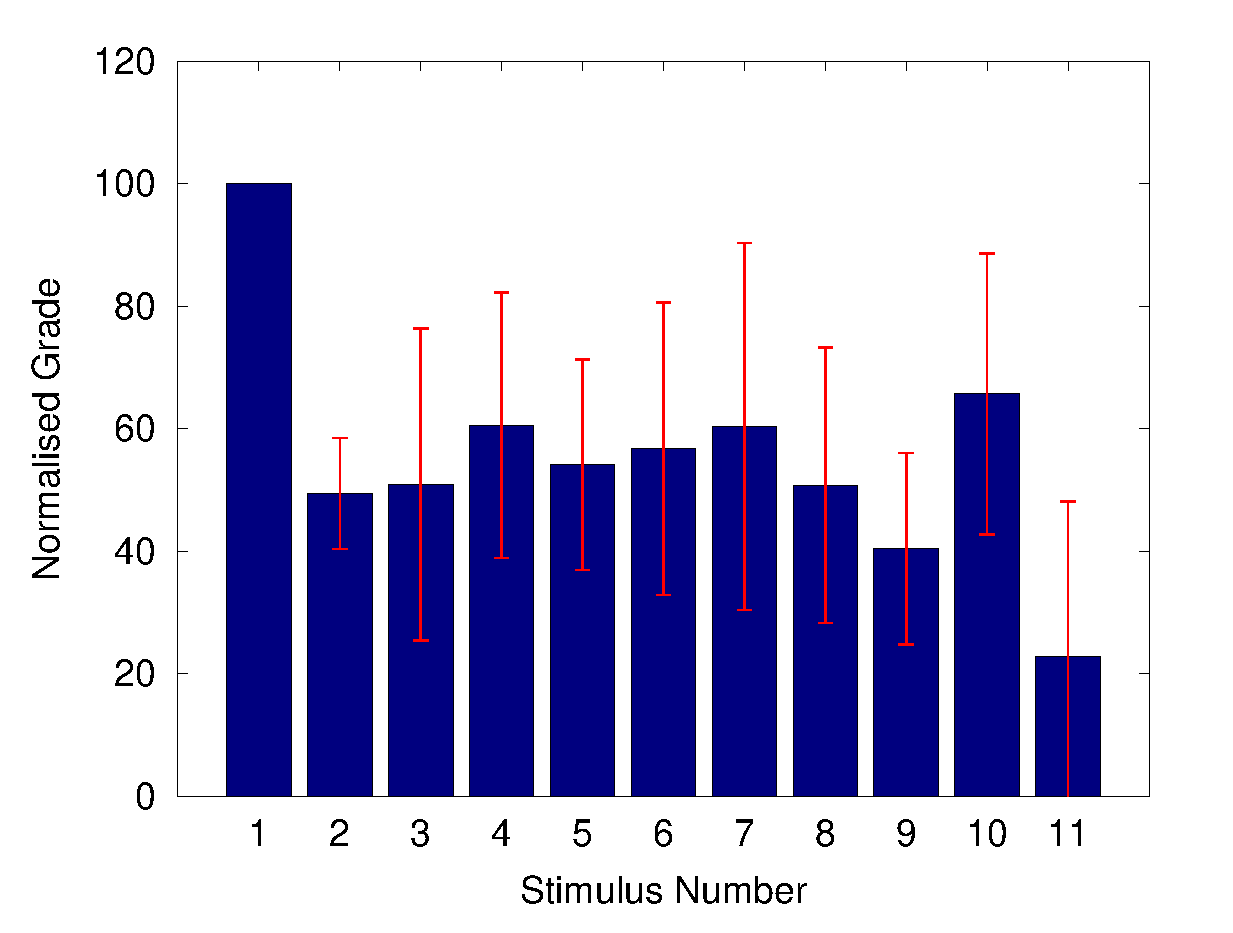
\includegraphics[width=0.45\textwidth]{chapter7/Images/SynthResults.eps}
			\label{fig:SynthResults}
		}
		\qquad
		\subfloat[Piano Sample]
		{
			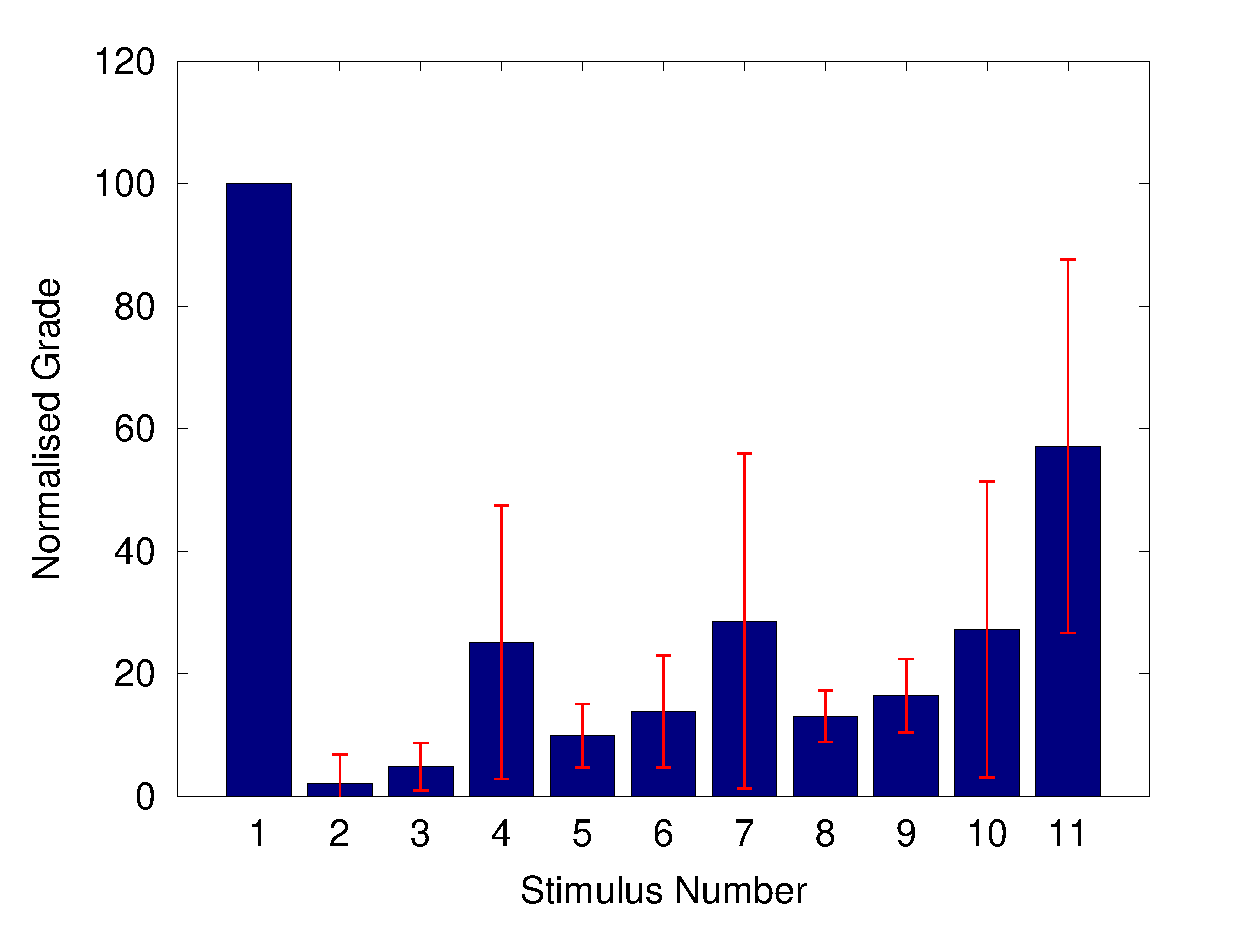
\includegraphics[width=0.45\textwidth]{chapter7/Images/PianoResults.eps}
			\label{fig:PianoResults}
		}
		\caption{Mean grades and confidence intervals for each of the stimuli.}
		\label{fig:SMCResults}
	\end{figure}

	Across all the samples there is a general increase in the perceived quality of the reproduction as the filter order
	or STFT window length is increased. With the SSBA and IAP methods increasing the filter order increases the level
	difference between the fundamental and its harmonics, better isolating the fundamental.  This is turn reduces the
	levels of intermodulation distortion in the output producing a `cleaner' harmonic.  With the synthesis method
	increasing the STFT window length increases the frequency resolution allowing for the amplitude envelope of the
	fundamental frequency to be measured more precisely.

	The piano sample used had very little energy at its fundamental frequency. This illustrates the problem discussed
	previously, there is not enough information in the amplitude envelope of the fundamental to reproduce the other
	harmonics. This leads to much lower grades for the reproduced signals than for any of the other samples. Figure
	\ref{fig:PianoResults} shows that the piano sample with its harmonics missing received a higher grade on average
	then any of the reconstructed samples further showing how poor the quality of the reconstructions is.

	The confidence intervals for the grades given to the majority of the stimuli are high. This is most likely due to
	there being too few participants in the experiment. To supplement these results each of the stimuli was graded with
	the R\sub{nonlin} metric. These results were normalised to the same range as the results from the listening test and
	are displayed in Figure \ref{fig:SMCRNonlin}.

	\begin{figure}[h!]
		\centering
		\subfloat[Cello Sample]
		{
			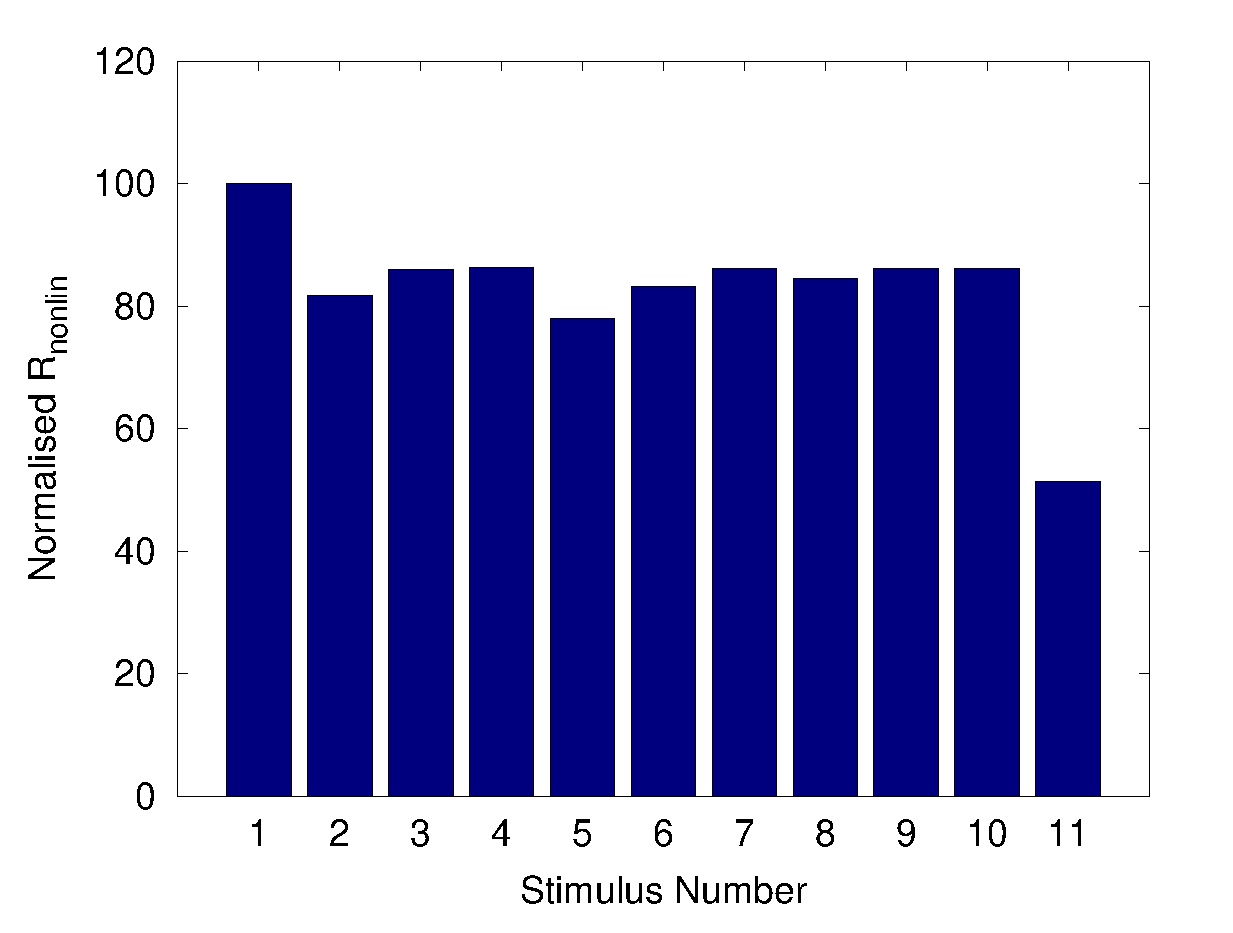
\includegraphics[width=0.45\textwidth]{chapter7/Images/CelloRNonlin.eps}
			\label{fig:CelloRNonlin}
		}
		\qquad
		\subfloat[Clarinet Sample]
		{
			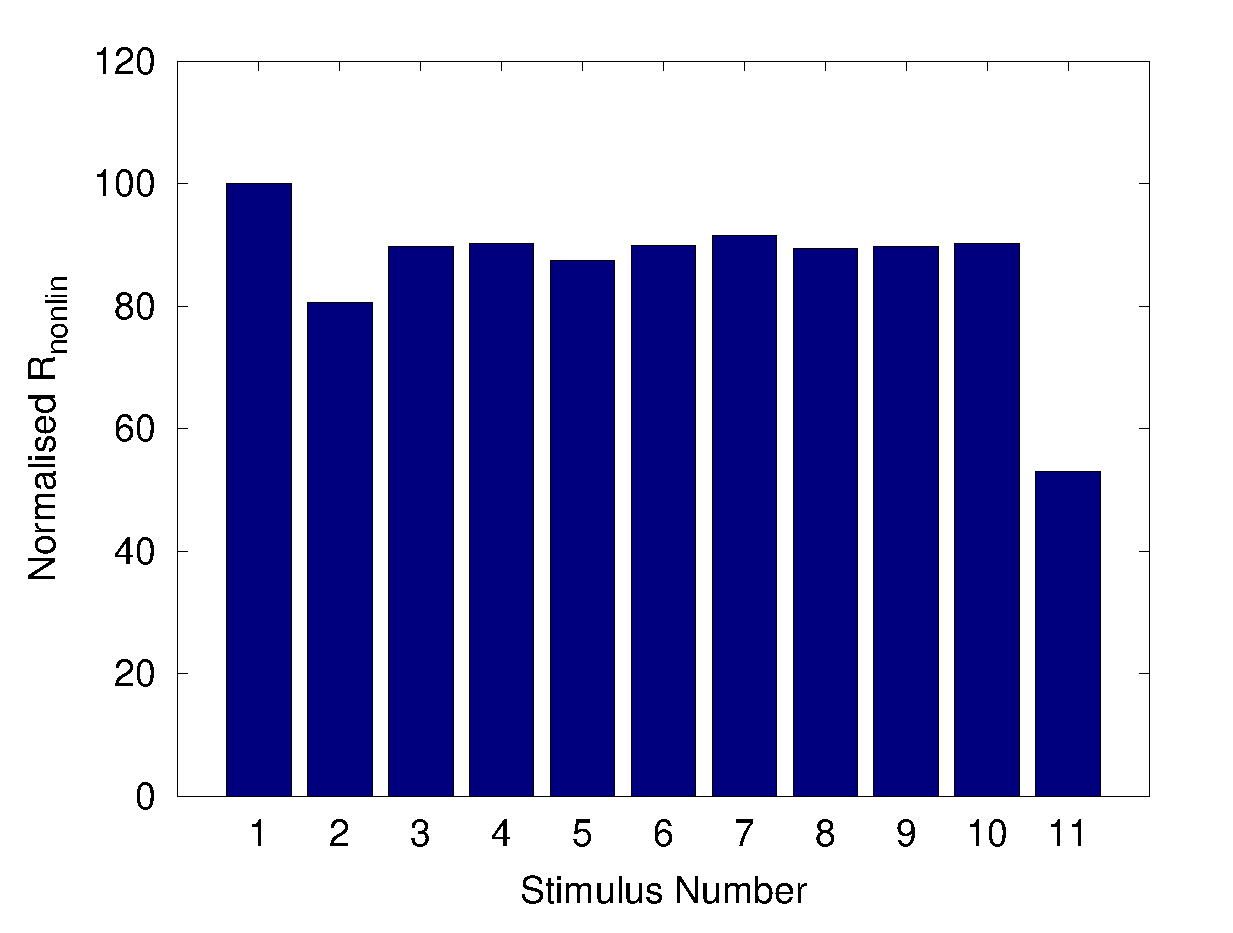
\includegraphics[width=0.45\textwidth]{chapter7/Images/ClarinetRNonlin.eps}
			\label{fig:ClarinetRNonlin}
		}

		\subfloat[Synthesised Sample]
		{
			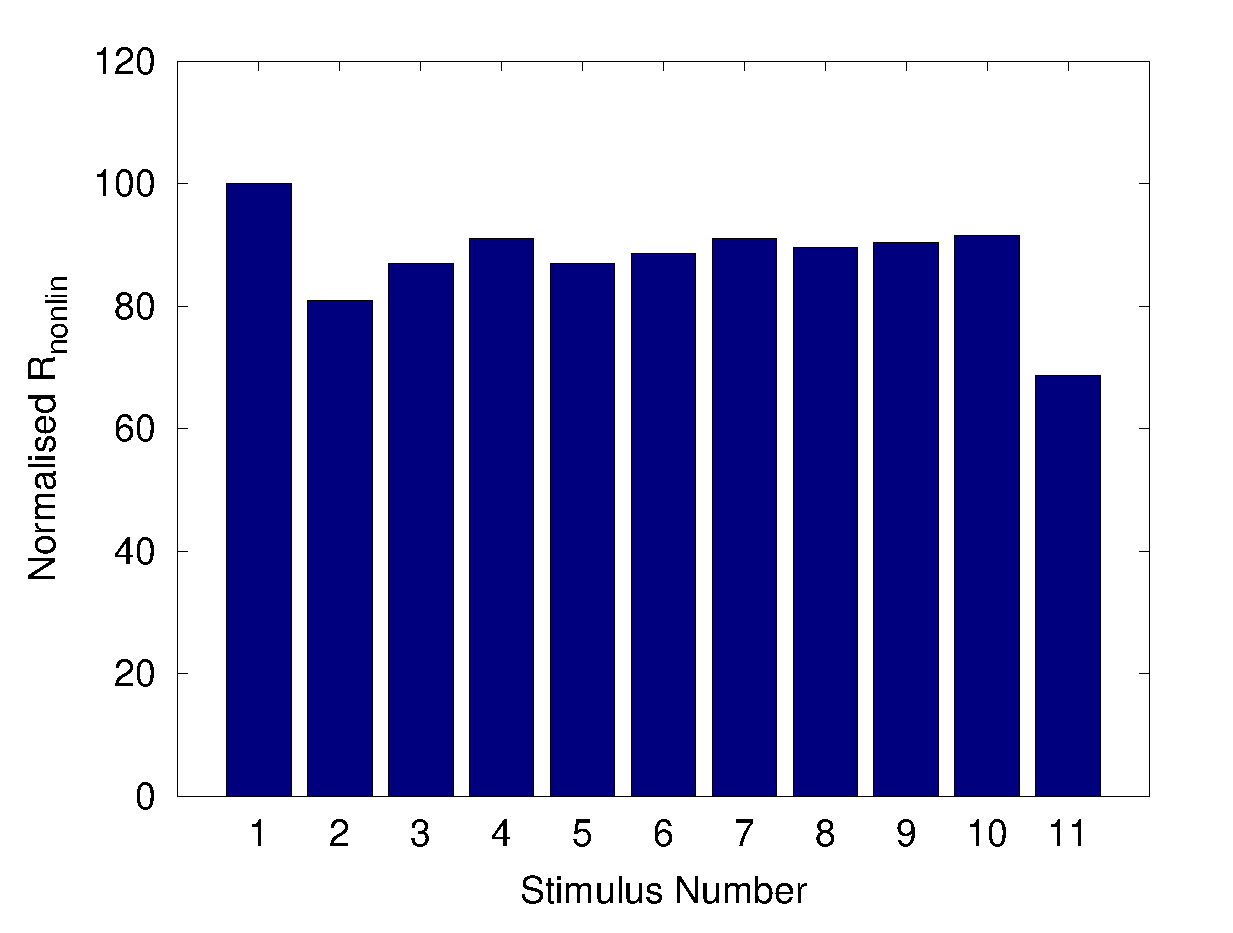
\includegraphics[width=0.45\textwidth]{chapter7/Images/SynthRNonlin.eps}
			\label{fig:SynthRNonlin}
		}
		\qquad
		\subfloat[Piano Sample]
		{
			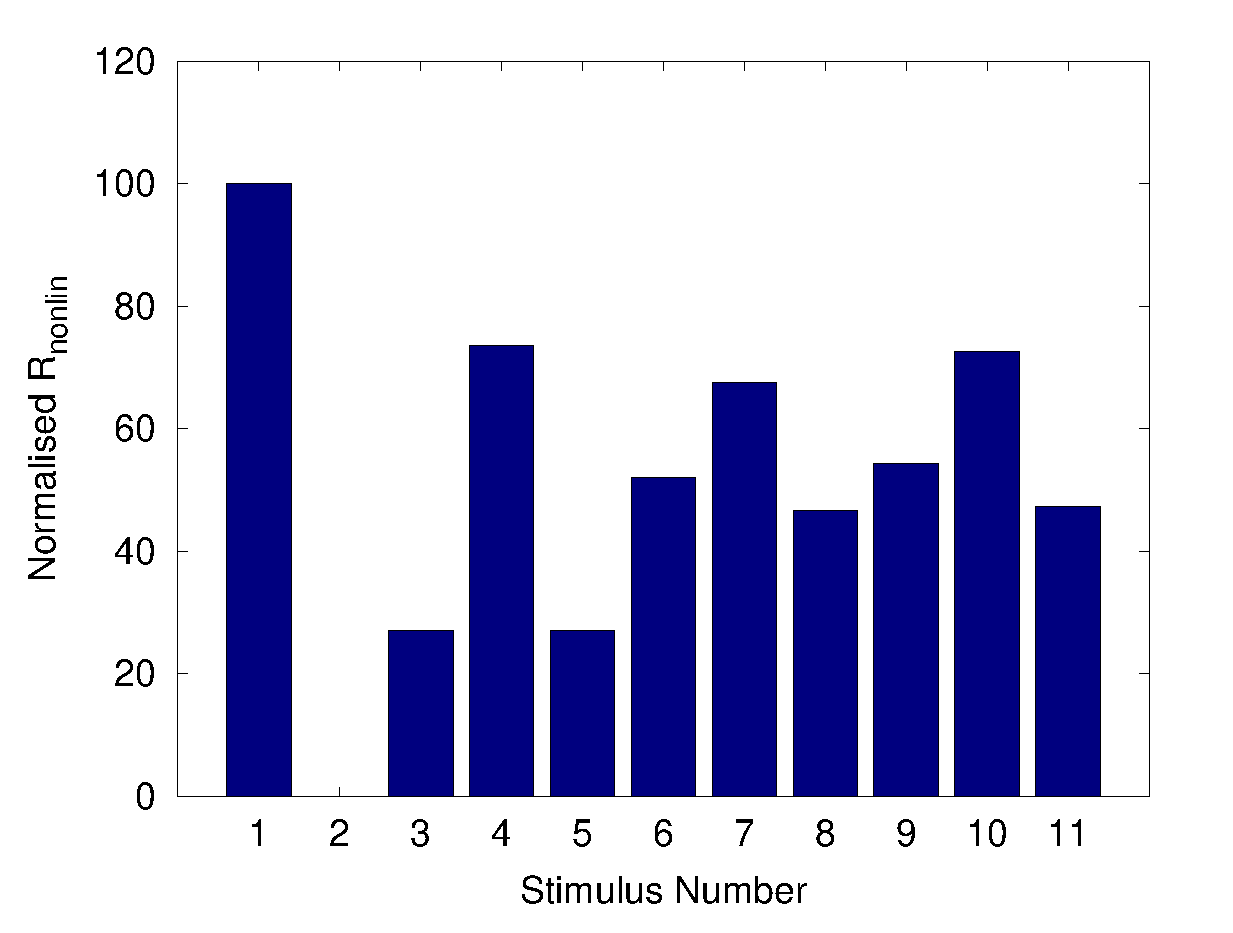
\includegraphics[width=0.45\textwidth]{chapter7/Images/PianoRNonlin.eps}
			\label{fig:PianoRNonlin}
		}
		\caption{R\sub{nonlin} values for each of the stimuli.}
		\label{fig:SMCRNonlin}
	\end{figure}

	The R\sub{nonlin} values support the correlations found in the listening test results. Using a higher order filter
	to isolate the fundamental improves the quality of the reconstruction. Figure \ref{fig:PianoRNonlin} again
	illustrates the problems which arise when the input signal has little energy at its fundamental frequency. Several
	of the reconstructions are objectively less similar to the original signal than the anchor stimulus.

	Both sets of results show that, using the highest order filter / STFT window lengths, each of the methods produce
	similar quality reconstructions of the original signal. For shorter filter lengths the IAP method provides more
	quality at then the SSBA method at the expense of requiring slightly more computation. The synthesis method produces
	similar quality results but incurs further computational complexity. 

	For timbral control applications the IAP method provides the greatest flexibility. For the majority of stimuli in
	this experiment it reproduced signals with the highest perceived quality. It was also shown in section
	\ref{sec:ExcitationEvaluation-Comparison-Homogeneity} that it is a homogeneous process allowing it to be applied to
	a wider range of signals with more predictable effects.

\section{Semantic Control}
\label{sec:PerceptualExperiments-SemanticControl}
